\chapter{Deisa}



\epigraph{\textit{If I have seen further, it is by standing on the shoulders of Giants.}} {Issac Newton}



\section{introduction}

\section{The Bridging Model between BSP and Task-Based Paradigms}

\subsection{Motivation}

\subsection{Terminology and Concepts}
 (task, EP, DF, deisa arrays)

 
\subsection{Producer Consumer Model}
 (to show the general architecture)



\section{Data Model}
\subsection{Data}
from ptr - pdi pybind -  pycall - numpy - dask

\subsection{Metadata}
what and how and why 
keys we get from a scatter, the size and position are sent 
used for dask array creation 
\subsection{Deisa virtual arrays}
from the simulation side as a mirror of the dask array that we create in the client side.

\section{Data and control communication}
\subsection{Control}
All control goes through the scheduler, but we can optimize it through mpi as future work 
\subsubsection{Queues} 

\subsubsection{Variables}
when several clients need the same data 

\subsection{Data communication}
\subsubsection{Deisa Bridge}
light client + far heartbeat 
limit 512 ..

\section{Data semantic}
in /out  data in a task vs same var and different values per time step in mpi

\section{Time-independent task submission}

\section{Steering}
limit generated data, but steering in the other sense can be done easily  
\subsection{Queues}
\subsection{Contracts}
\section{Dynamic scheduling}
triggers I have to do that 


\section{Implementation}

\cite{deisa}

\subsection{Architecture}
\begin{figure}[tb]\centering
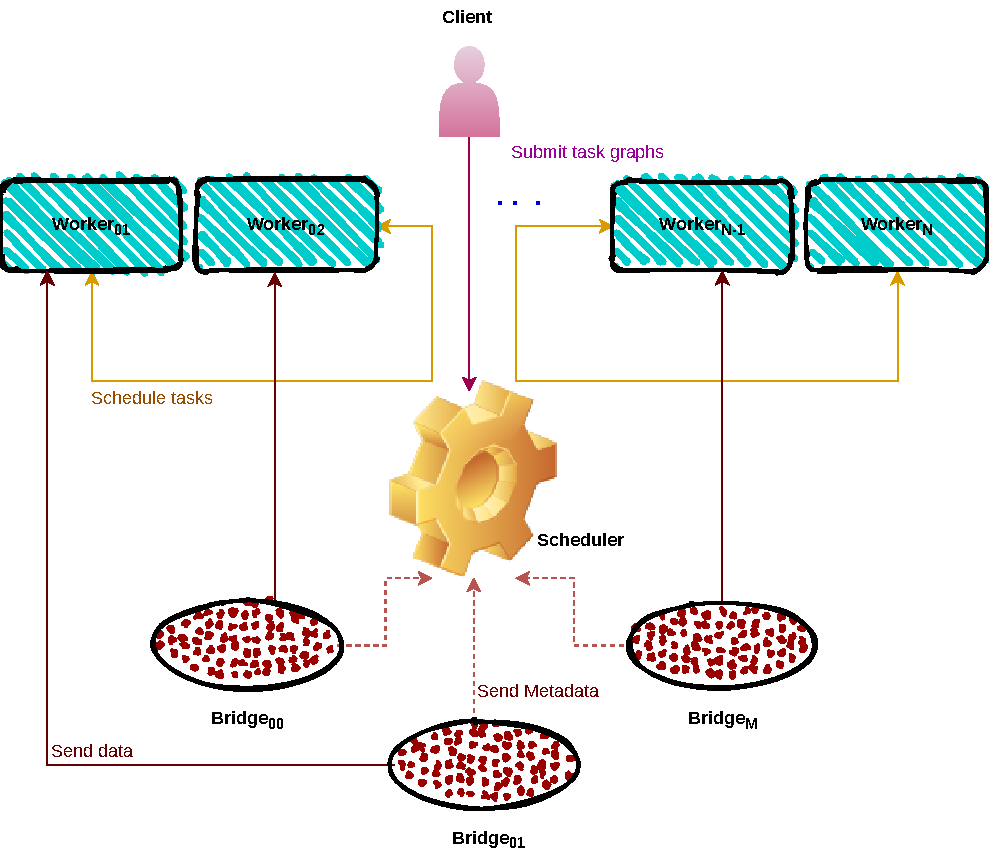
\includegraphics{figures/ArchiectureDeisa.pdf}
\caption{\deisa}
\label{figdeida}
\end{figure}

\begin{figure}[tb]\centering
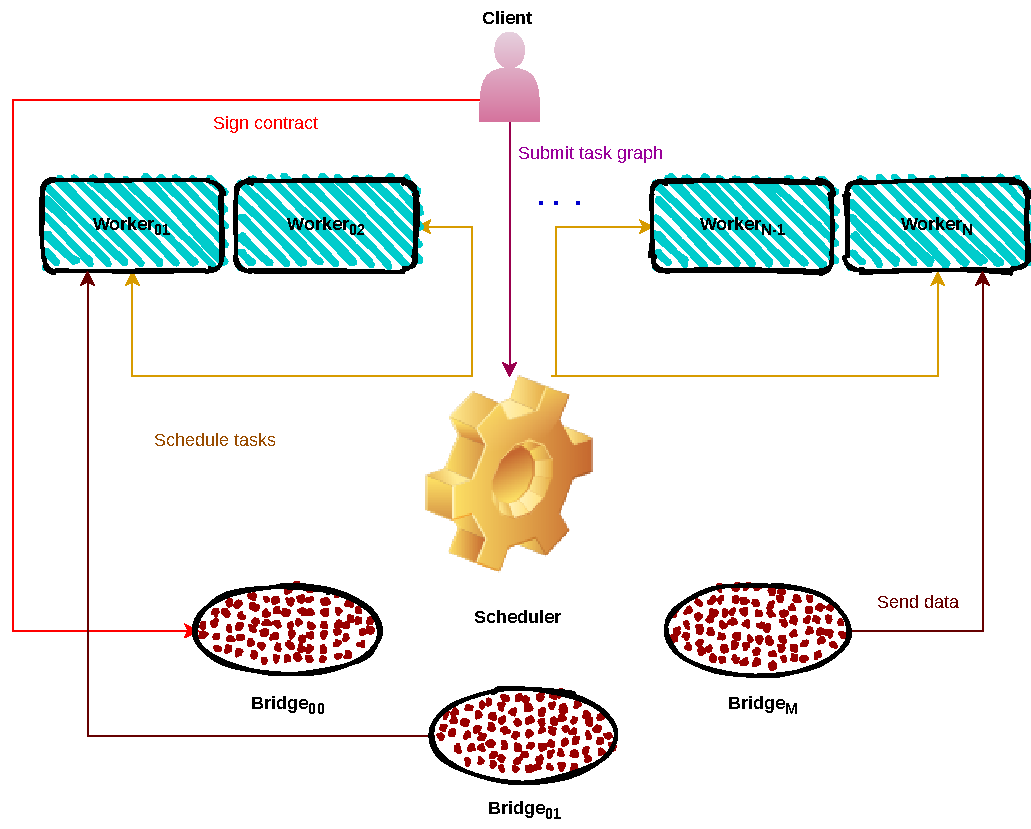
\includegraphics{figures/ArchiectureDeisaV2.pdf}
\caption{\deisa v2}
\label{figdeidav2}
\end{figure}
\subsection{API}
just the last one 
\subsection{Instrumentation}
\begin{lstlisting}[float, label=ymldata, language=yaml, caption=Data description in \pdi \deisa YAML file]
types: #[...] including config_t description
metadata: {step: int, cfg: config_t, rank: int} |\label{ymldata:metadata}|
data: 
plugins:
  mpi: # get MPI rand and size
  deisa:
    scheduler_info: scheduler.json
    init_on: init 
    time_step: $step 
    deisa_arrays: # Deisa Virtual arrays
      G_temp: # Field name
        type: array
        subtype: double
        size:
          -timedim 
          -'$cfg.loc[0] * ($rank % $cfg.proc[0])'
          -'$cfg.loc[1] * ($rank / $cfg.proc[0])'
        subsize: [1, '$cfg.loc[0]', '$cfg.loc[1]'] # chunk size
        start:  # chunk start
          -$step
          -'$cfg.loc[0] * ($rank % $cfg.proc[0])'
          -'$cfg.loc[1] * ($rank / $cfg.proc[0])'
        +timedim: 0 # a tag for the time dimension
    map_in: # deisa array mapping
      temp: G_temp
        
\end{lstlisting}
\subsection{Evaluation}
\subsection{Limitations}

\section{Conclusion}